\documentclass[../main.tex]{subfiles}

\begin{document}

\section{Fysica voorbij het Standaard Model}%
\label{sec:fysica_voorbij_het_standaard_model}

\subsection{Het standaard Model: wat zit daar nu allemaal in?}%
\label{sub:het_standaard_model_wat_zit_daar_nu_allemaal_in_}

\begin{equation}
    \begin{aligned}
        \label{eq:standaard_model}
            \begin{array}{ccc}
                \left(\begin{array}{c}
                        \nu_{e} \\
                        e
                        \end{array}\right) & \left(\begin{array}{c}
                        \nu_{\mu} \\
                        \mu
                        \end{array}\right) & \left(\begin{array}{c}
                        \nu_{\tau} \\
                        \tau
                \end{array}\right) \\
                \left(\begin{array}{l}
                        u \\
                        d
                        \end{array}\right) & \left(\begin{array}{l}
                        c \\
                        s
                        \end{array}\right) & \left(\begin{array}{l}
                        t \\
                        b
                \end{array}\right)
            \end{array}\\
            \gamma, W^{+}, W^{-}, Z, g, H
    \end{aligned}
\end{equation}
Dit zijn alle deeltjes die nodig hebben om het Standaard Model te laten werken. Deze zijn ook allemaal gevonden.\\
Waarom beperken we ons hier tot 4 generaties (Dit moet omdat de $CP$ schending niet meer zou kloppen), zijn er nog andere uitwisselingdeeltjes, zijn er nog andere interacties, zijn er parameters die we nog niet kennen?

\subsection{4de generatie fermionen}%
\label{sub:4de_generatie_fermionen}

\subsubsection{Leptonen}%
\label{ssub:leptonen}

Indien we een vierde generatie leptonen zouden hebben zou de massa van de 4de generatie groter moeten zijn dan $45$GeV. Voor de geladen leptonen weten we dat $m_l > 101$GeV omdat we nog geen resonantie zijn tegen gekomen in $e^{+} e^{-} \rightarrow l^{+} l^{-}$ tot $\sqrt{s}=209 \mathrm{GeV}$.

\subsubsection{Quarks}%
\label{ssub:quarks}

Uit de unitariteit van de CKM-matrix is het duidelijk dat daar niet veel zal zitten. We doen hier ook direct onderzoek naar op het LHC maar er is nog niets gevonden.

\begin{figure}[h]
    \centering
    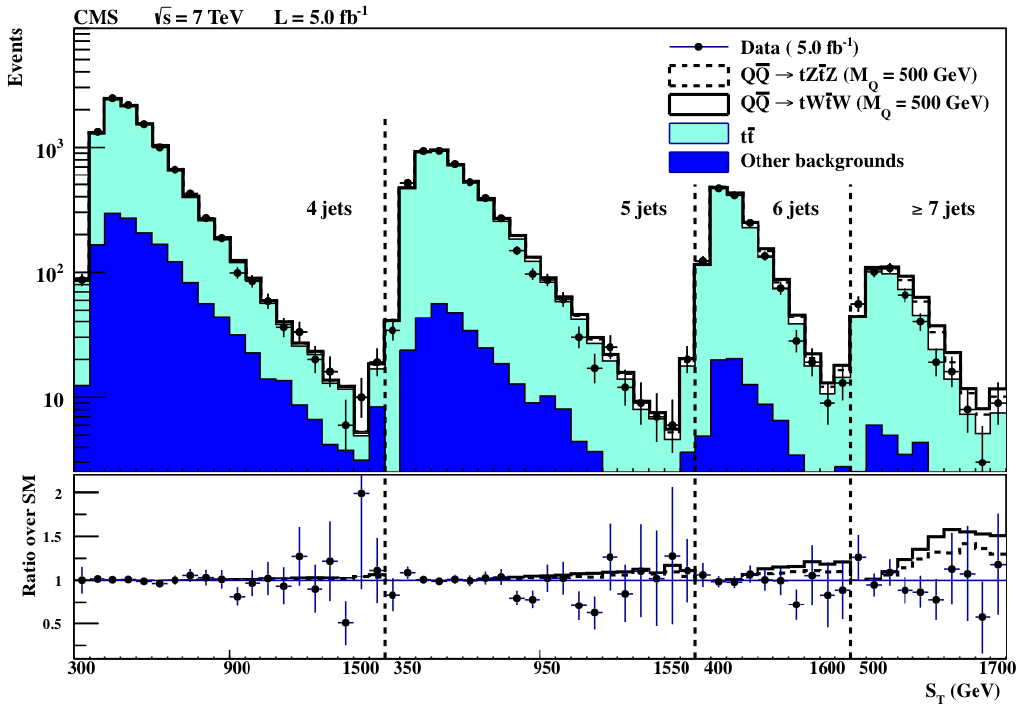
\includegraphics[width=0.6\linewidth]{physics_beyond_the_standard_model/lhc_4_gen_zoektocht.png}
    \caption{Zoektocht naar 4de generatie quarks in LHC}%
    \label{fig:physics_beyond_the_standard_model/lhc_4_gen_zoektocht}
\end{figure}

Uit de proton proton botsingen kunnen zowel 4, 5, 6 of 7 jets komen. Berekenen we alle mogelijke productie kanalen van deze jets zien we dat we bij de metingen niet echt afwijken van de voorspellingen. Er zit daar dus niet echt een 4de generatie aan quarks.

\subsection{Nieuwe uitwisseling bosonen}%
\label{sub:nieuwe_uitwisselings_bosonen}

Waarom zouden er geen extra $W'$ en $Z'$ bosonen bestaan. Misschien koppelen deze aan rechtshandige fermionen. Wie weet is $Z$ een samengestelde toestand en is daar een aangeslagen toestand van.

\begin{figure}[h]
    \centering
    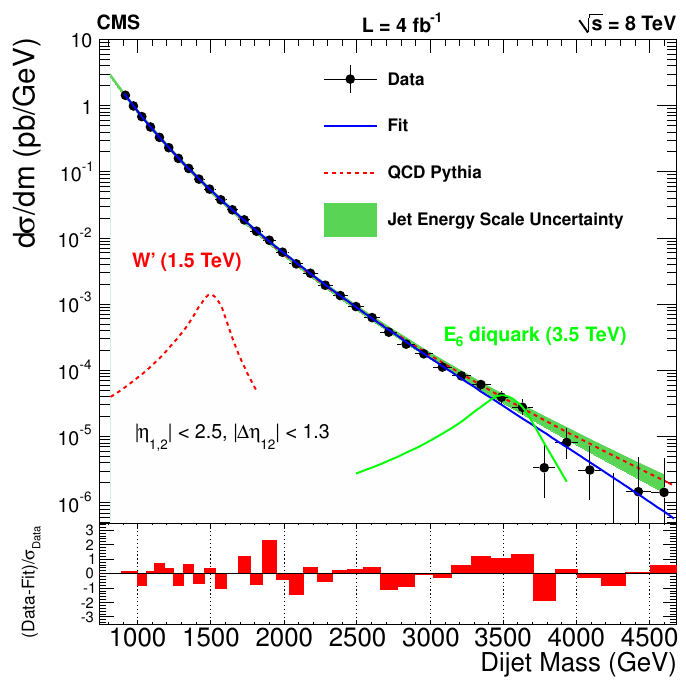
\includegraphics[width=0.4\linewidth]{physics_beyond_the_standard_model/cms_w'_z'_zoektocht.png}
    \caption{Zoektocht naar $W'$ en $Z'$ in LHC}%
    \label{fig:physics_beyond_the_standard_model/cms_w'_z'_zoektocht}
\end{figure}

We gaan kijken hier naar 2 jet fenomenen waar we hun gecombineerde massa uitzetten in vergelijking tot de werkzame doorsnede. De groene lijn is wat we verwachten en de blauwe lijn is wat we meten. We zien hier niet de spectra indien een $W'$ of diquark zou bestaan. Er is dus geen ruimte om af te wijken van het standaard model hier. Hetzelfde kunnen we vinden als we kijken naar de elektron positron vervallen. Er is hier ook geen plaats om de nieuwe intermediaire deeltjes toe te voegen aan het model.

\begin{figure}[h]
    \centering
    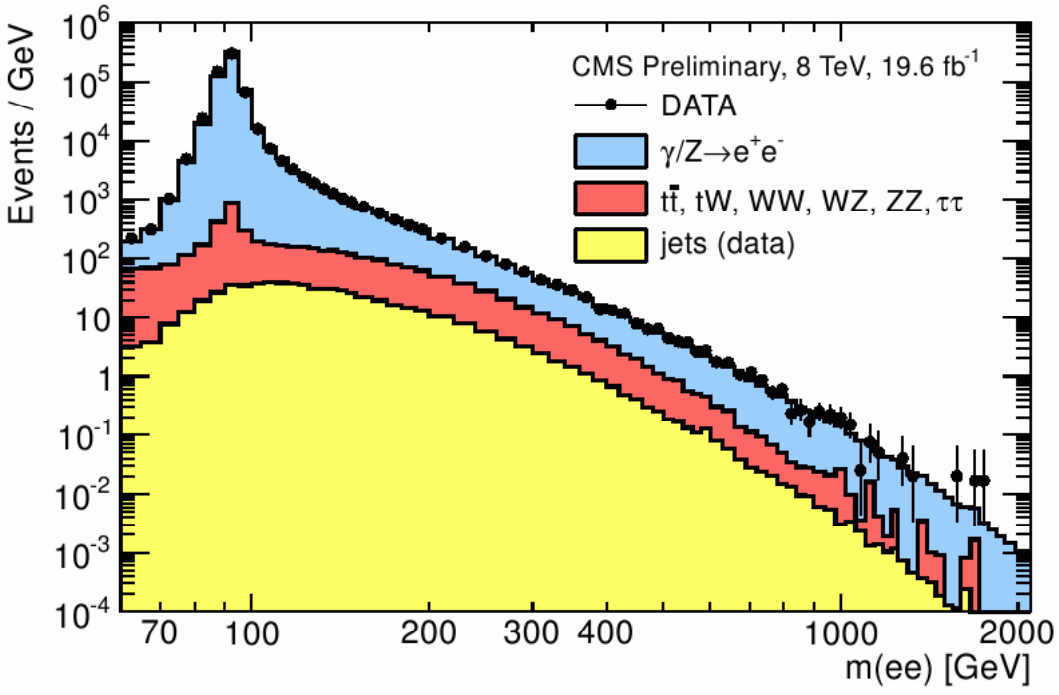
\includegraphics[width=0.6\linewidth]{physics_beyond_the_standard_model/ee_w'_z'_zoektocht.png}
    \caption{Zoektocht naar $W'$ en $Z'$ in LHC aan de hand van elektronen en positronen}%
    \label{fig:physics_beyond_the_standard_model/ee_w'_z'_zoektocht}
\end{figure}

\subsection{Zwarte gaten}%
\label{sub:zwarte_gaten}

Het is nu ook mogelijk om te zoeken naar zwarte gaten. Deze worden voorspelt door string theory. Deze voorspelt dat er nog veel meer dimensies zijn. In de opgerolde dimensies zou de zwaartekracht veel groter moeten zijn. Indien we deze dimensies zouden beginnen raken als we onze deeltjes maar dicht genoeg tot elkaar brengen zou het mogelijk moeten zijn om mini zwarte gaten te kunnen maken.
\begin{equation}
    \begin{aligned}
        \label{eq:zwarte_gaten}
        p p \rightarrow B H+X
    \end{aligned}
\end{equation}
Deze zijn heel klein en zouden zo goed als instant vervallen (verdampen) aan de hand van Hawking radiatie. Bij het maken van deze zwarte gaten zou een hoge multipliciteit aan finale toestanden moeten zijn van veel jets en leptonen. Om dit te onderzoeken kijken we of we zo evenementen kunnen vinden met grote jet aantallen.
\begin{figure}[h]
    \centering
    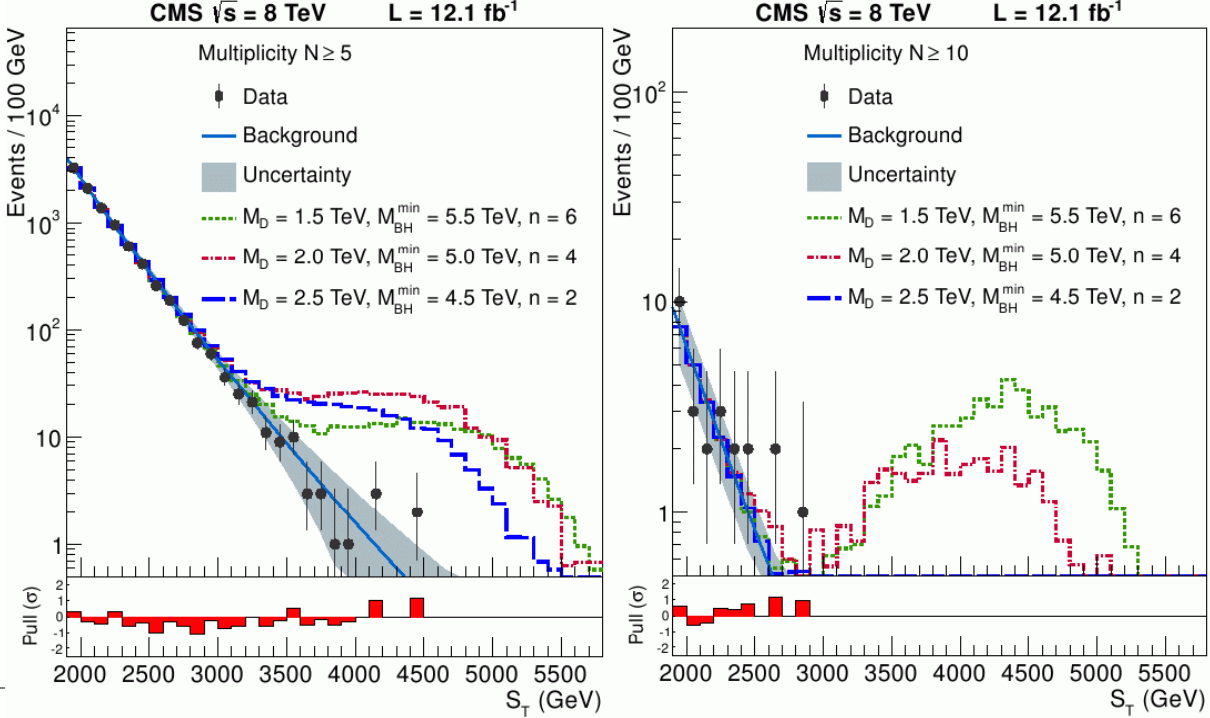
\includegraphics[width=0.6\linewidth]{physics_beyond_the_standard_model/zwarte_gaten.png}
    \caption{Zoektocht naar zwarte gaten}%
    \label{fig:physics_}
\end{figure}

In het blauw kan je de verwachtingen zien wat perfect zal kloppen met wat we zien. Indien we zwarte gaten zouden hebben met de massa's gegeven in de grafieken zouden we een grotere hoeveelheid aan evenementen verwachten bij grote $S_T$.

\end{document}
